\subsection{Màn hình Menu của Server}
\subsubsection{Mô tả}
Dưới đây là nội dung hiển thị của màn hình Menu tương ứng với vai trò \textbf{User} (\textbf{Server}). Vì \textbf{Server} chỉ có vai trò gửi nhận và thực hiện các yêu cầu mà \textbf{Client} gửi đến, do đó ở màn hình Menu ứng dụng chỉ hỗ trợ 1 chức năng đó là khởi động \textbf{Server} để chờ kết nối đến từ \textbf{Client} (nút \textbf{Start Listening}). (Hình \ref{fig:ServerMenuWindow})
\begin{figure}[H]
	\centering{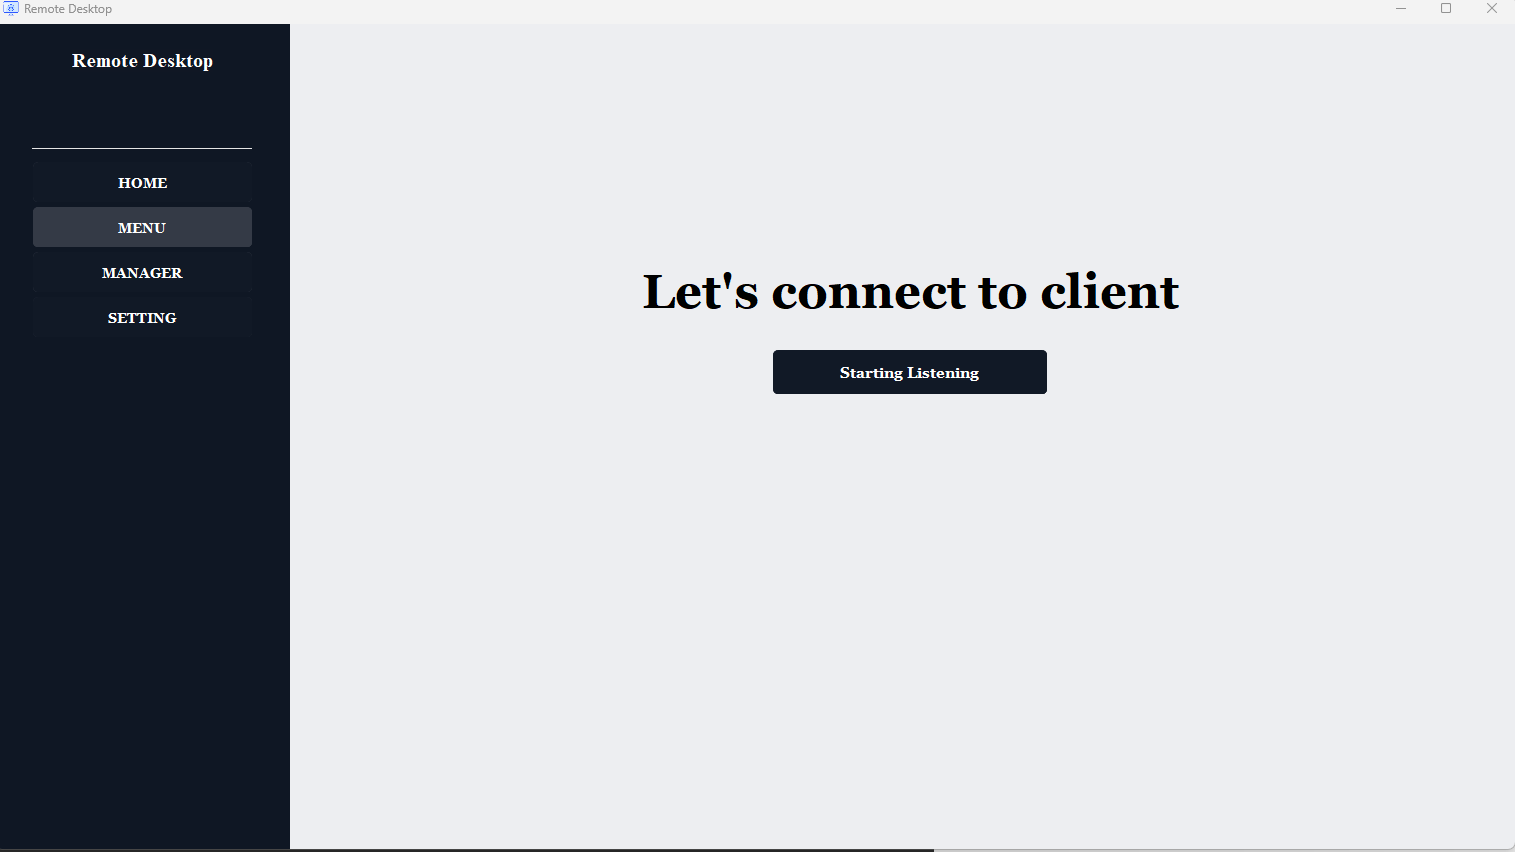
\includegraphics[scale=0.4]{ServerMenuWindow}}
	\caption{Màn hình Menu ứng với vai trò User thông thường (Server)}
	\label{fig:ServerMenuWindow}
\end{figure}

\subsubsection{Chờ kết nối từ Client (Nút Start Listening)}
%\subsubsection{Hướng dẫn sử dụng}
Khi ta ấn vào nút \textbf{Start Listening}, một cửa sổ với tiêu đề là \textbf{Server Window} hiện lên. Đây là cửa sổ text hiển thị tình trạng của \textbf{Server}, ở trạng thái ban đầu cửa sổ sẽ hiển thị mỗi dòng chữ ``Server is running''. (Hình \ref{fig:ServerLoggerWindow})
\begin{figure}[H]
	\centering{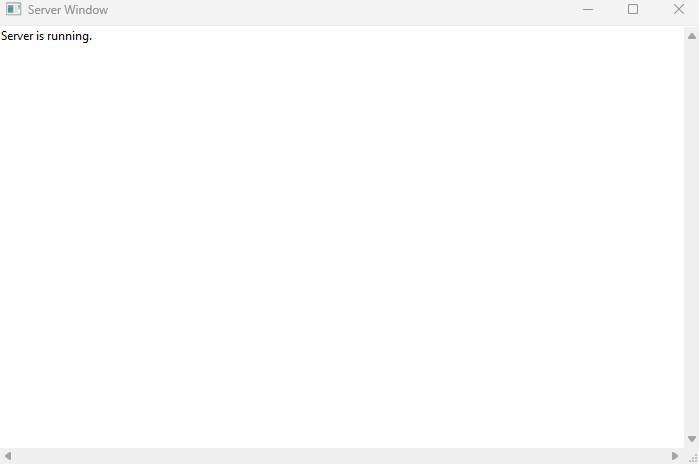
\includegraphics[scale=0.75]{ServerLoggerWindow}}
	\caption{Cửa sổ Server Window lúc đầu}
	\label{fig:ServerLoggerWindow}
\end{figure}

Nếu có \textbf{Client} kết nối đến \textbf{Server}, khi đó cửa sổ \textbf{Server Window} sẽ thông báo là Client đã kết nối đến Server thông qua dòng chữ ``A client has connected to server!'' và theo sau là những thông tin cơ bản về địa chỉ IP, địa chỉ MAC và tên cửa sổ gửi tín hiệu kết nối của Client. Ở trong hình bên dưới, Server hiển thị 2 dòng chữ đã kết nối vì bên phía Client thiết lập 2 kết nối đến Server, một cái dùng để nhận hình ảnh màn hình từ phía Server và cái còn lại dùng để gửi tín hiệu điều khiển đến máy Server. (Hình \ref{fig:ServerWindowConnected})
\begin{figure}[H]
	\centering{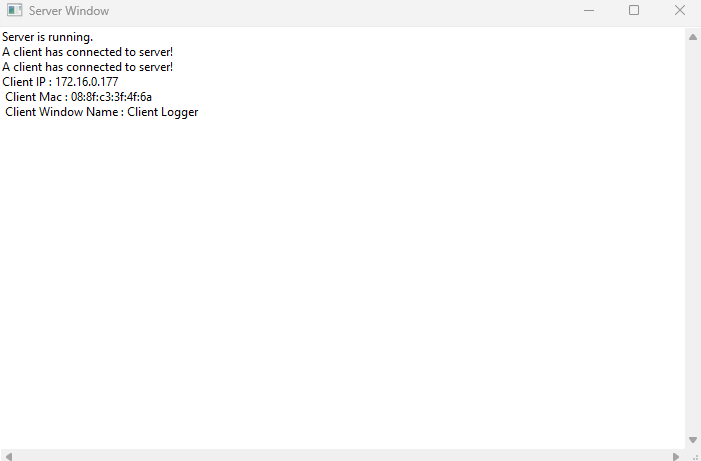
\includegraphics[scale=0.75]{ServerWindowConnected}}
	\caption{Cửa sổ Server Window khi có kết nối đến từ Client}
	\label{fig:ServerWindowConnected}
\end{figure}

\subsubsection{Tắt Server}
Để tắt Server, ta chỉ cần nhấn vào nút \textbf{X} ở góc phải trên của cửa sổ, khi ta nhấn vào nút này thì một hộp thoại sẽ hiển thị để yêu cầu ta xác nhận về việc có đóng cửa sổ ``Server Window'' và đồng thời tắt Server luôn hay không (Hình \ref{fig:ServerClosingDialog}). 

\begin{figure}[H]
	\centering{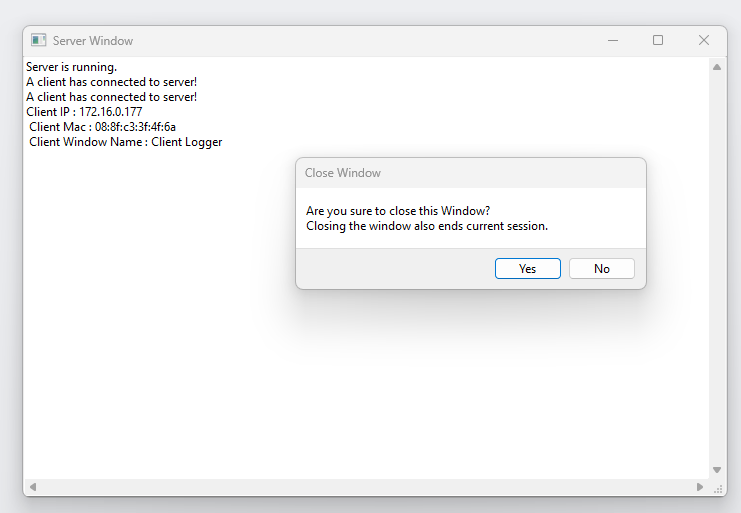
\includegraphics[scale=0.75]{ServerClosingDialog}}
	\caption{Hộp thoại đóng/tắt Server}
	\label{fig:ServerClosingDialog}
\end{figure}

Nếu ta chọn \textbf{No}, Server vẫn tiếp tục hoạt động bình thường còn nếu ta chọn \textbf{Yes}, Server sẽ gửi thông báo đến Client về việc ngắt kết nối và yêu cầu Client ngắt toàn bộ các kết nối đã thiết lập với Server, sau đó Server mới tắt hẳn. Sau khi Server gửi yêu cầu ngắt kết nối đến Client thành công, cửa sổ Client sẽ ngắt các kết nối mà nó đã thiết lập với Server và một thông báo sẽ hiện ra ở bên máy của Client như sau (Hình \ref{fig:DisconnectedFromServer}):

\begin{figure}[H]
	\centering{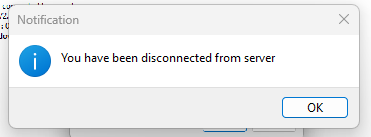
\includegraphics[scale=1]{DisconnectedFromServer}}
	\caption{Thông báo ở máy Client sau khi Server đóng}
	\label{fig:DisconnectedFromServer}
\end{figure}

